\documentclass[12pt,a4paper]{article}

% ─── Packages ─────────────────────────────────────────────────────────────────
\usepackage[utf8]{inputenc}
\usepackage[T1]{fontenc}
\usepackage{amsmath,amssymb}
\usepackage{geometry}
\geometry{margin=2.5cm}
\usepackage{setspace}
\onehalfspacing
\usepackage{booktabs}
\usepackage{longtable}
\usepackage{graphicx}
\usepackage{float}
\usepackage{hyperref}
\usepackage{natbib}
\usepackage{caption}
\usepackage{pdflscape}
\usepackage{multirow}
\usepackage{array}
\usepackage{listings}
\usepackage{xcolor}

\lstset{
  language=R,
  basicstyle=\ttfamily\footnotesize,
  breaklines=true,
  frame=single,
  backgroundcolor=\color{gray!5},
  commentstyle=\color{green!50!black},
  keywordstyle=\color{blue},
  stringstyle=\color{red!70!black},
  numbers=left,
  numberstyle=\tiny\color{gray},
  numbersep=5pt
}

\hypersetup{
  colorlinks=true,
  linkcolor=blue,
  citecolor=blue,
  urlcolor=blue
}

% ═══════════════════════════════════════════════════════════════════════════════
% TITLE PAGE
% ═══════════════════════════════════════════════════════════════════════════════
\title{\textbf{Determinants of Protest Violence: \\ What Makes Mass Demonstrations Turn Violent?}}
\author{Kamilla Tadjibaeva, Nijat Kazimli \\ MSc Economics -- Econometrics Project}
\date{June 2026}

\begin{document}
\maketitle

% ═══════════════════════════════════════════════════════════════════════════════
% ABSTRACT
% ═══════════════════════════════════════════════════════════════════════════════
\begin{abstract}
\noindent \textbf{Aims:} This paper investigates which observable characteristics of mass demonstrations---their size, duration, stated demands, and the state's prior behaviour---predict whether a protest event will turn violent.

\noindent \textbf{Method:} We employ a binary logit model estimated on 15,239 protest events from the Mass Mobilization dataset (166 countries, 1990--2020). Variable selection follows the LSE General-to-Specific (G2S) methodology, reducing a General Unrestricted Model of 51 regressors to a parsimonious specification of 35 coefficients including two interaction terms. All inference uses country-clustered standard errors.

\noindent \textbf{Main findings:} Cumulative state repression is the dominant predictor of protest violence (marginal effect: $+35.8$ percentage points, $p < 0.001$). Demand type is the second major driver---protests demanding police accountability ($+32.9$pp, $p < 0.001$) and price relief ($+22.6$pp, $p < 0.001$) carry the highest violence risk. The interaction between police demands and cumulative state violence is negative ($-28.3$pp, $p < 0.05$), indicating that the demand effect attenuates in already-repressive contexts. Despite modest overall fit (McFadden $R^2 = 0.066$), all key results are statistically robust.
\end{abstract}

\newpage
\tableofcontents
\newpage

% ═══════════════════════════════════════════════════════════════════════════════
\section{Introduction}
% ═══════════════════════════════════════════════════════════════════════════════

Mass demonstrations are a fundamental mechanism of political expression in both democratic and authoritarian regimes. Yet a substantial fraction of protests turns violent, with consequences ranging from personal injury and property destruction to broader political destabilisation. Understanding the determinants of this transition from peaceful to violent protest is critical for conflict prevention, policy design, and the protection of civil liberties.

This paper asks: \emph{What observable characteristics of protests, their demands, their context, and the state's prior behaviour predict whether a mass demonstration will become violent?}

\subsection{Hypotheses}

We formulate one main hypothesis and several secondary hypotheses:

\paragraph{Main hypothesis.}
\textbf{H1 (State violence drives escalation):} The state's history of violent repression---both cumulative and recent---is the dominant predictor of whether protesters resort to violence. Countries with a long track record of repressive state responses trap subsequent protests in an escalation cycle.

\paragraph{Secondary hypotheses.}
\begin{itemize}
  \item \textbf{H2 (Demand type matters):} The specific grievances articulated by protesters (police accountability, prices, land, corruption, political reform, labour) jointly predict protest violence, with confrontational demands (police brutality) carrying the highest risk.
  \item \textbf{H3 (Regional variation):} Geographic context significantly influences violence probability, even after controlling for protest-level characteristics, reflecting unobserved institutional differences.
  \item \textbf{H4 (Temporal shocks):} Global shocks (economic crises, waves of democratisation) shift the baseline violence propensity across years.
  \item \textbf{H5 (Protest scale):} Protest size, duration, and their interaction affect violence risk---larger protests may be marginally less violent, but prolonged large protests face compounding escalation pressures.
\end{itemize}

\subsection{Importance of the Topic}

Understanding what makes protests turn violent has direct policy relevance. If state repression is the dominant escalation mechanism, then de-escalation policies focused on changing state behaviour can be more effective than reactive crowd-control measures. Identifying which demand types carry higher violence risk allows targeted institutional responses that address root grievances before confrontation occurs.

% ═══════════════════════════════════════════════════════════════════════════════
\section{Literature Review}
% ═══════════════════════════════════════════════════════════════════════════════

The study of protest violence sits at the intersection of contentious politics, conflict studies, and political economy. Several theoretical traditions inform our empirical strategy.

\paragraph{Escalation and repression.}
The ``escalation trap'' or ``protest--repression nexus'' literature argues that state violence begets protester violence. \citet{davenport2007} documents that repression can radicalise movements, while \citet{lichbach1987} formalises the strategic interaction between states and challengers. Recent empirical work by \citet{ritter2015} confirms that prior repression significantly predicts subsequent protest intensity. Our inclusion of both a one-period lag and a cumulative running mean of state violence directly operationalises this theoretical mechanism.

\paragraph{Grievance type and framing.}
The ``framing'' approach to contentious politics \citep{benford2000} suggests that how grievances are articulated affects tactical choices. Protests framing their demands in directly confrontational terms (e.g., against police brutality) may attract violence-prone participants or trigger harsher police responses. \citet{wilkes2006} finds that grievance type conditions the relationship between mobilisation and outcomes.

\paragraph{Protest size and collective action.}
The relationship between protest size and violence is theoretically ambiguous. Larger crowds may benefit from ``safety in numbers'' and stronger self-policing \citep{biggs2018}, but may also overwhelm police capacity and create anonymity that reduces individual accountability \citep{granovetter1978}. Our log-transformation and large-protest indicator allow both mechanisms to operate.

\paragraph{Cross-national event data.}
The Mass Mobilization dataset \citep{clark2020mass} enables cross-national comparison at the event level, overcoming the limitations of single-country case studies. Similar datasets (GDELT, ACLED) have been used to study conflict dynamics, but MM provides uniquely detailed demand-level coding for protests specifically.

% ═══════════════════════════════════════════════════════════════════════════════
\section{Data}
% ═══════════════════════════════════════════════════════════════════════════════

\subsection{Data Source}

We use the Mass Mobilization (MM) dataset, version July 31, 2020 \citep{clark2020mass}, available through the Harvard Dataverse. The dataset records protest events globally with information on participants, demands, state responses, and outcomes.

\subsection{Sample Construction}

After restricting to observations where \texttt{protest == 1} (excluding non-protest entries such as strikes without public mobilisation), our analytic sample comprises:
\begin{itemize}
  \item \textbf{15,239 protest events}
  \item \textbf{166 countries}
  \item \textbf{Period: 1990--2020}
\end{itemize}

\subsection{Dependent Variable}

The binary outcome variable \texttt{protesterviolence} equals 1 if protesters engaged in violence during the event and 0 otherwise. In our sample, approximately \textbf{26.4\%} of protests involved protester violence (roughly 4,023 events).

\subsection{Data Transformations}

\paragraph{Protest size.}
Two source columns exist in the raw data: a bucketed \texttt{participants\_category} (e.g., ``100--999'', ``1000--1999'') and a free-text \texttt{participants} field. We harmonise both into a single numeric \texttt{protest\_size} by:
\begin{enumerate}
  \item Assigning category midpoints (e.g., ``100--999'' $\to$ 550, ``$>$10000'' $\to$ 15000).
  \item Parsing the free-text field (handling numeric suffixes like ``1000s'').
  \item Preferring the bucketed estimate; falling back to the parsed value.
  \item Imputing remaining missing values by country-specific median (with global median fallback).
  \item Creating an explicit binary indicator \texttt{protest\_size\_missing} for imputed observations.
\end{enumerate}
The resulting variable exhibits heavy right-skew, motivating a log-transformation: $\texttt{log\_protest\_size} = \ln(\texttt{protest\_size} + 1)$.

\paragraph{Duration.}
Computed as the difference between end and start dates in days. Negative values (data errors) are set to zero.

\paragraph{Demand dummies.}
Up to four free-text demand fields per event are collapsed into seven binary topic indicators via keyword matching (e.g., \texttt{demand\_police} flags mentions of ``police'' or ``brutal''). A count variable \texttt{n\_demands} records the total number of distinct demands (1--4).

\paragraph{State violence history.}
We construct two lag variables within each country (ordered chronologically):
\begin{itemize}
  \item \texttt{lag1\_state\_violence}: Did the state use violence in the immediately preceding event?
  \item \texttt{cum\_state\_violence}: Cumulative running mean of state violence \emph{before} the current event (avoiding information leakage).
\end{itemize}
For the first event per country (no prior history), both are set to 0.

\paragraph{Removed observations.}
No observations are dropped beyond the initial \texttt{protest == 1} filter. All missing values are resolved by construction (imputation with indicator, lag initialisation to 0). A missingness sanity check confirms zero NAs across all columns.

\subsection{Exploratory Data Analysis}

\paragraph{Violence by region.}
Violence rates vary substantially across regions: Africa and South America exhibit the highest shares of violent protests, while Europe and MENA show lower rates conditional on protest occurrence.

\begin{figure}[H]
\centering
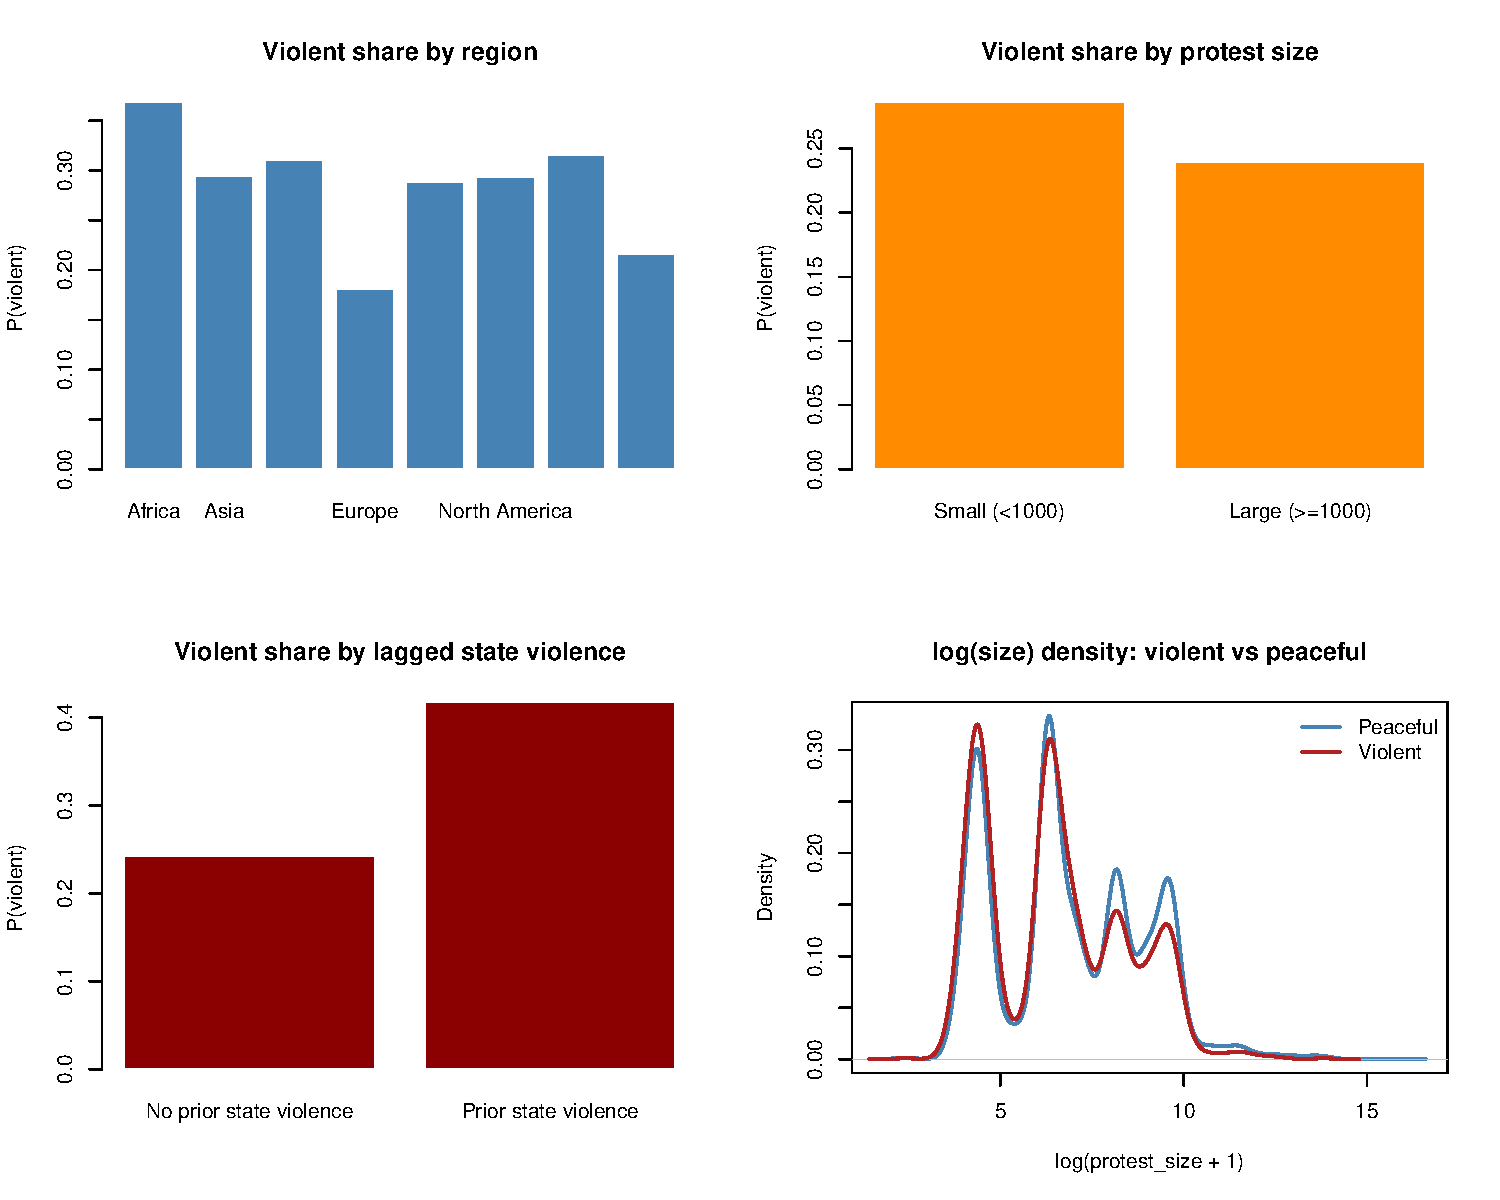
\includegraphics[width=0.95\textwidth]{figures/outcome_vs_regressors.pdf}
\caption{Bivariate associations with protest violence. Violence shares differ across regions and are markedly higher when the previous event in the same country involved state violence; larger (log) protests are also distributed differently between violent and peaceful events.}
\label{fig:outcome-regressors}
\end{figure}

\paragraph{Violence by state history.}
Protests preceded by state violence in the previous event show markedly higher violence rates than those without such precedent, providing preliminary visual evidence for the escalation hypothesis.

\begin{figure}[H]
\centering
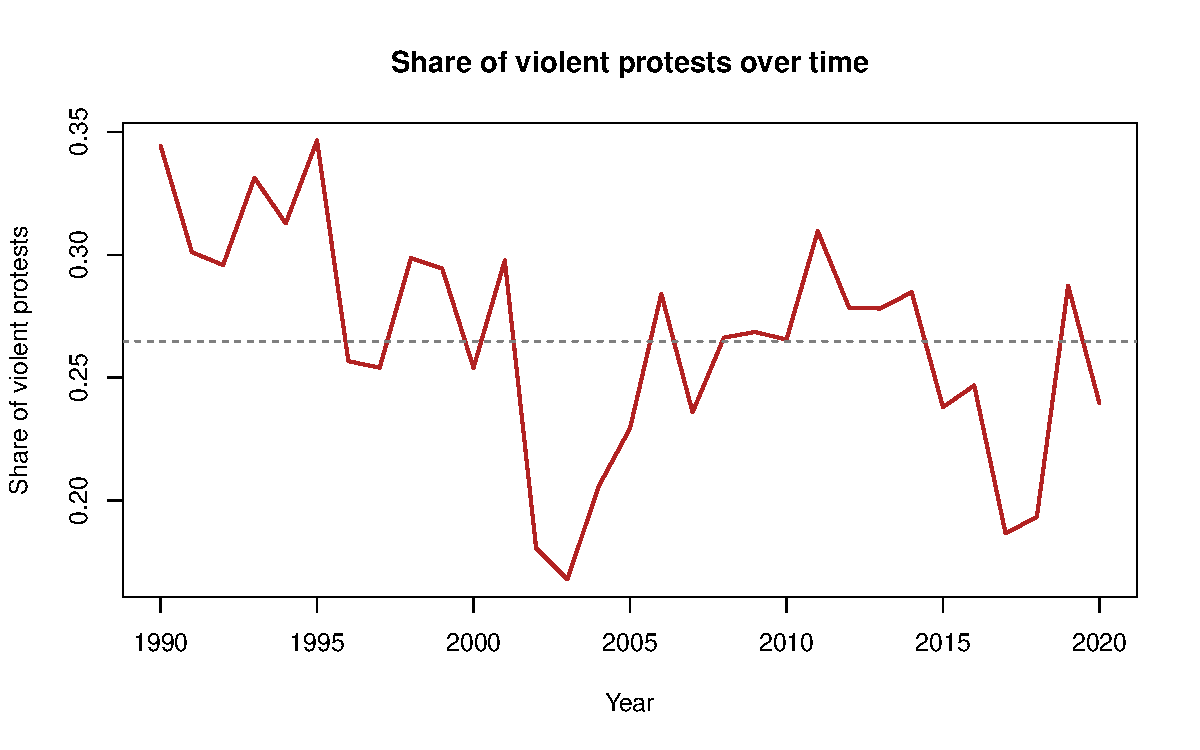
\includegraphics[width=0.85\textwidth]{figures/violence_by_year.pdf}
\caption{Share of violent protests by year, 1990--2020. Year-to-year variation around the global mean motivates the inclusion of year fixed effects.}
\label{fig:violence-year}
\end{figure}

\paragraph{Size distribution.}
The raw protest size distribution is extremely right-skewed (median $\approx$ 550, with outliers above 15,000). The log-transformation produces an approximately symmetric distribution, supporting its use in the regression.

\begin{figure}[H]
\centering
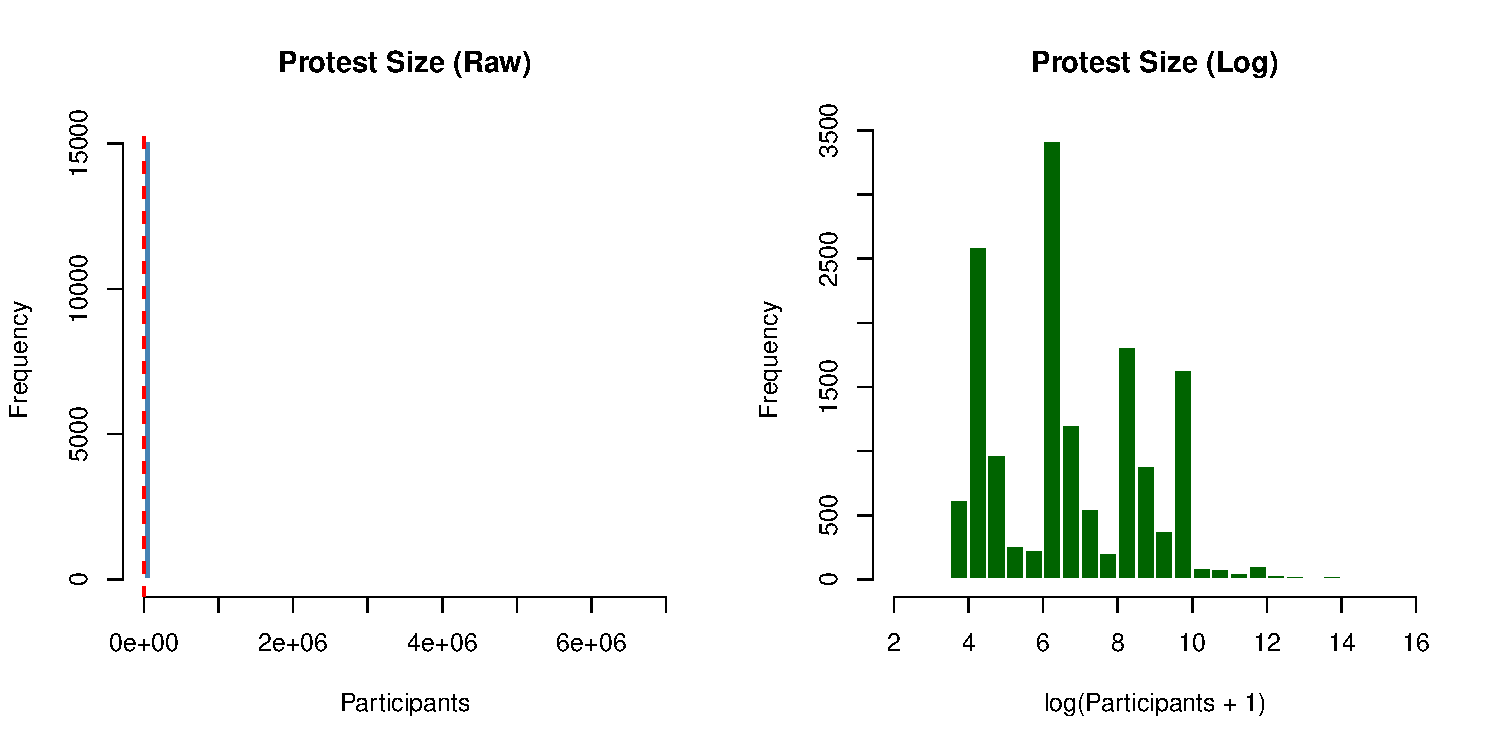
\includegraphics[width=0.9\textwidth]{figures/protest_size_distribution.pdf}
\caption{Distribution of protest size. Left: raw participants count is heavily right-skewed. Right: after the $\ln(\text{size}+1)$ transformation the distribution is approximately symmetric, justifying the use of \texttt{log\_protest\_size} in the regression.}
\label{fig:size-dist}
\end{figure}

\paragraph{Multicollinearity.}
Variance inflation factors (VIFs) computed on a preliminary linear model are all below conventional thresholds (max VIF $< 5$), confirming that multicollinearity is not a concern for our candidate regressors.

\begin{figure}[H]
\centering
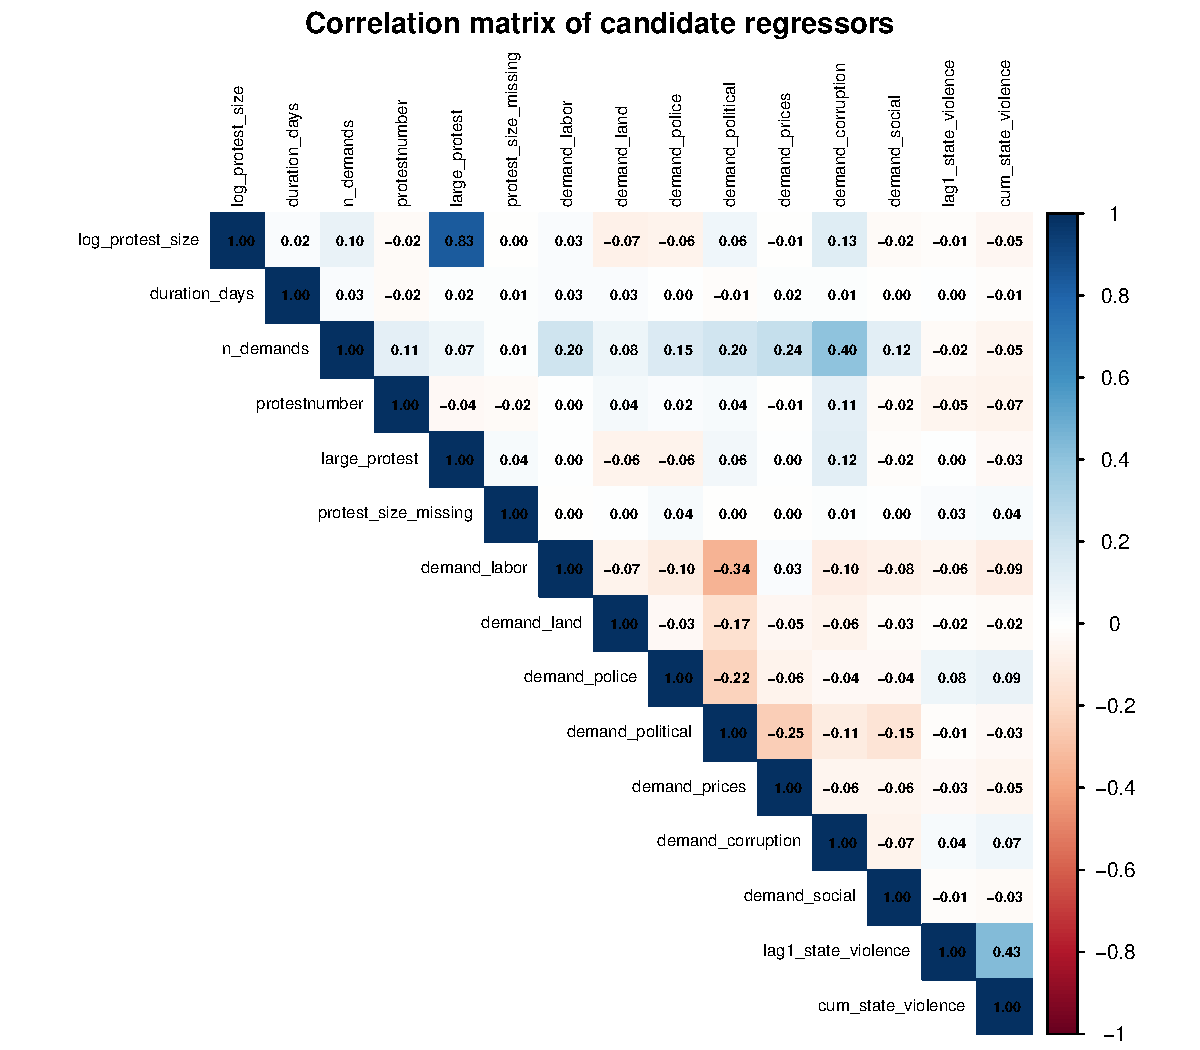
\includegraphics[width=0.8\textwidth]{figures/correlation_matrix.pdf}
\caption{Spearman correlation matrix of candidate regressors and the outcome. No pair exhibits correlation strong enough to threaten identification, consistent with the VIF diagnostic.}
\label{fig:corr-matrix}
\end{figure}

% ═══════════════════════════════════════════════════════════════════════════════
\section{Method / Model}
% ═══════════════════════════════════════════════════════════════════════════════

\subsection{Model Specification}

Given the binary nature of the dependent variable, we estimate a logistic regression:
\begin{equation}
  P(y_i = 1 \mid \mathbf{x}_i) = \Lambda(\mathbf{x}_i' \boldsymbol{\beta})
  = \frac{\exp(\mathbf{x}_i' \boldsymbol{\beta})}{1 + \exp(\mathbf{x}_i' \boldsymbol{\beta})}
\end{equation}
where $\Lambda(\cdot)$ is the logistic CDF and $\mathbf{x}_i$ includes all covariates described above.

\subsection{Link Function Selection: Logit vs Probit}

Before beginning variable selection, we compare the logit and probit link functions on the full General Unrestricted Model (GUM) using information criteria:
\begin{itemize}
  \item \textbf{AIC}: Logit is lower (preferred).
  \item \textbf{BIC}: Logit is lower (preferred).
\end{itemize}
\textbf{Decision:} Both criteria favour the logit. We proceed with $\text{link} = \text{logit}$ for all subsequent estimation.

\subsection{General-to-Specific (G2S) Variable Selection}

We follow the LSE (Hendry) General-to-Specific protocol, as demonstrated in Lab~08:

\begin{enumerate}
  \item \textbf{Start from the GUM}: Include all theoretically motivated regressors (51 coefficients: 15 scalar covariates + 7 region dummies + 30 year dummies, excluding the baseline categories).
  \item \textbf{Read cluster-robust $p$-values}: At each step, identify insignificant variables via \texttt{coeftest} with \texttt{vcovCL} (clustered by country).
  \item \textbf{Batch test}: Propose dropping all currently insignificant scalars simultaneously. Test joint insignificance against the GUM via likelihood ratio (LR) test.
  \begin{itemize}
    \item If $p > 0.05$: fail to reject $H_0$ (dropped variables are jointly insignificant) $\Rightarrow$ proceed with elimination.
    \item If $p \leq 0.05$: reject $H_0$ (at least one dropped variable is needed) $\Rightarrow$ switch to individual elimination.
  \end{itemize}
  \item \textbf{Individual elimination}: Remove the single most insignificant variable, re-test the cumulative set of all dropped variables against the GUM.
  \item \textbf{Stopping rule}: Stop when the next variable to drop causes the joint test to reject at $\alpha = 0.05$.
\end{enumerate}

\subsubsection{G2S Elimination Steps}

\paragraph{Step 1: GUM $\to$ gum1 (batch drop of 12 variables).}
We identify 12 insignificant variables: \texttt{demand\_social}, \texttt{region\_oceania}, and 10 year dummies (1993, 1994, 1995, 1998, 1999, 2001, 2006, 2009, 2014, 2019).\\
LR test against GUM: $p > 0.05$. \textbf{Fail to reject $H_0$}---they are jointly insignificant. We drop all 12.

\paragraph{Step 2: gum1 $\to$ gum2 (batch drop of 3 variables).}
Newly insignificant: \texttt{year\_1991}, \texttt{year\_1992}, \texttt{year\_2020}.\\
LR test against GUM: $p > 0.05$. \textbf{Fail to reject $H_0$.} We drop all 3.

\paragraph{Step 3: gum2 $\to$ gum3 (batch drop of 2 variables).}
Newly insignificant: \texttt{year\_1996}, \texttt{year\_2008}.\\
LR test against GUM: $p > 0.05$. \textbf{Fail to reject $H_0$.} We drop both.

\paragraph{Step 4: gum3 $\to$ gum4 (batch drop of 4 variables---REJECTED).}
Attempted: \texttt{year\_2007}, \texttt{year\_2011}, \texttt{year\_2013}, \texttt{year\_2018}.\\
LR test against GUM: $p \leq 0.05$. \textbf{Reject $H_0$}---at least one of these is needed. We revert to one-at-a-time elimination starting from gum3.

\paragraph{Step 5: gum3 $\to$ gum5 (individual drop).}
Drop the most insignificant variable: \texttt{year\_2013}.\\
Joint test of all variables dropped so far against GUM: $p > 0.05$. \textbf{Fail to reject.} We drop \texttt{year\_2013}.

\paragraph{Step 6: gum5 $\to$ gum6 (individual drop).}
Drop the most insignificant: \texttt{year\_2011}.\\
Joint test: $p > 0.05$. \textbf{Fail to reject.} We drop \texttt{year\_2011}.

\paragraph{Step 7: gum6 $\to$ gum7 (individual drop).}
Drop the most insignificant: \texttt{year\_2007}.\\
Joint test: $p > 0.05$. \textbf{Fail to reject.} We drop \texttt{year\_2007}.

\paragraph{Step 8: gum7 $\to$ STOP.}
Attempted to drop \texttt{year\_2018}.\\
Joint test of all cumulative drops including \texttt{year\_2018}: $p \leq 0.05$. \textbf{Reject $H_0$}---\texttt{year\_2018} is needed. We stop the G2S process.

\paragraph{Final G2S model (\texttt{gum7}).}
The surviving specification retains \textbf{33 coefficients} (including intercept): 10 scalar regressors (\texttt{log\_protest\_size}, \texttt{large\_protest}, \texttt{protest\_size\_missing}, \texttt{duration\_days}, \texttt{protestnumber}, \texttt{n\_demands}, \texttt{lag1\_state\_violence}, \texttt{cum\_state\_violence}), 6 demand dummies, 6 region dummies, and 12 year dummies.

\subsection{Specification Testing and Interaction Terms}
\label{sec:interactions}

\subsubsection{Linktest on gum7}

We apply the Pregibon linktest to the G2S model. Under correct specification, the linear predictor $\hat{y}$ should be significant while $\hat{y}^2$ should not:
\begin{itemize}
  \item $\hat{y}$: coefficient significant, $p < 2 \times 10^{-16}$. \checkmark
  \item $\hat{y}^2$: coefficient $= -0.151$, $p = 4.24 \times 10^{-7}$. \textbf{Significant---indicates misspecification.}
\end{itemize}

\textbf{Interpretation:} The significant $\hat{y}^2$ term suggests the model is missing nonlinear terms or interaction effects. The negative sign indicates the true probability curve is less steep than the logit predicts in certain regions of the index.

\subsubsection{What We Did to Address Misspecification}

To address the linktest failure, we introduced theoretically motivated interaction terms. The rationale: if the index function is misspecified due to omitted nonlinearities, adding interactions between variables that plausibly interact can improve the specification. We tested three candidates:

\paragraph{Interaction 1: \texttt{large\_protest} $\times$ \texttt{lag1\_state\_violence}.}
\emph{Theory}: The escalation effect of recent state violence may differ by protest size (large protests may be harder to provoke).\\
\emph{Result}: Coefficient $p = 0.81$. \textbf{Not significant---we reject this interaction.} It does not improve the specification, and we do not include it in the final model.

\paragraph{Interaction 2: \texttt{cum\_state\_violence} $\times$ \texttt{demand\_police}.}
\emph{Theory}: Protests demanding police accountability in countries with high cumulative state repression may face a qualitatively different violence dynamic (ceiling effect or tactical adaptation).\\
\emph{Result}: Coefficient $p = 6.07 \times 10^{-5}$. \textbf{Highly significant---we retain this interaction.}

\paragraph{Interaction 3: \texttt{log\_protest\_size} $\times$ \texttt{duration\_days}.}
\emph{Theory}: Large protests that persist over multiple days face compounding escalation pressures (fatigue, provocation, logistical breakdown).\\
\emph{Result}: Coefficient $p = 5 \times 10^{-6}$. \textbf{Highly significant---we retain this interaction.}

\subsubsection{Linktest After Adding Interactions}

After adding the two significant interactions, we re-run the linktest on the augmented model:
\begin{itemize}
  \item $\hat{y}$: $p < 2 \times 10^{-16}$. \checkmark
  \item $\hat{y}^2$: coefficient shrinks from $-0.151$ to $\mathbf{-0.084}$; $p$-value weakens from $4.24 \times 10^{-7}$ to $\mathbf{2.08 \times 10^{-5}}$.
\end{itemize}

\textbf{Assessment:} The misspecification signal is substantially reduced (coefficient halved, $p$-value weakened by two orders of magnitude) but not fully eliminated ($p = 2.08 \times 10^{-5}$ still rejects at 5\%). The remaining signal likely reflects unobserved heterogeneity inherent in cross-country event data (police tactics on the day, protest leadership quality, media presence) that cannot be captured with available observables. We acknowledge this as a model limitation but proceed given: (a) the substantial improvement over the base model, (b) the Osius--Rojek goodness-of-fit test passing comfortably (see Section~\ref{sec:gof}).

\subsubsection{Final Model}

The final model contains \textbf{35 coefficients}: 33 from G2S + 2 interaction terms:
\begin{equation}
\begin{split}
P(\text{violence}_i = 1) = \Lambda\Big( & \beta_0 + \beta_1 \cdot \text{log\_size}_i + \beta_2 \cdot \text{large\_protest}_i + \beta_3 \cdot \text{size\_missing}_i \\
& + \beta_4 \cdot \text{duration}_i + \beta_5 \cdot \text{demand\_political}_i + \ldots + \beta_{10} \cdot \text{demand\_corruption}_i \\
& + \beta_{11} \cdot \text{n\_demands}_i + \beta_{12} \cdot \text{protestnumber}_i \\
& + \beta_{13} \cdot \text{lag1\_state\_violence}_i + \beta_{14} \cdot \text{cum\_state\_violence}_i \\
& + \sum_r \gamma_r \cdot \text{region}_{ri} + \sum_t \delta_t \cdot \text{year}_{ti} \\
& + \beta_{33} \cdot (\text{cum\_state\_violence}_i \times \text{demand\_police}_i) \\
& + \beta_{34} \cdot (\text{log\_size}_i \times \text{duration}_i) \Big)
\end{split}
\end{equation}

\subsection{Inference}

All standard errors throughout the paper are clustered at the country level using the sandwich estimator (\texttt{vcovCL} from the \texttt{sandwich} package). This accounts for arbitrary within-country correlation across protest events---critical since protests within the same country share institutional, cultural, and historical contexts that induce dependence.

% ═══════════════════════════════════════════════════════════════════════════════
\section{Results}
% ═══════════════════════════════════════════════════════════════════════════════

\subsection{Overall Model Significance: LR Test vs Null}

We test whether the final model as a whole is statistically significant by comparing it to a null (intercept-only) model via the likelihood ratio test:
\begin{itemize}
  \item $H_0$: All 34 slope coefficients are jointly zero ($\beta_1 = \beta_2 = \ldots = \beta_{34} = 0$).
  \item $H_1$: At least one slope coefficient $\beta_k \neq 0$.
  \item \textbf{Test statistic}: $\chi^2(34) = 1{,}167.5$.
  \item \textbf{$p$-value}: $< 2.2 \times 10^{-16}$.
  \item \textbf{Decision}: We \textbf{reject $H_0$} at any conventional significance level ($\alpha = 0.01, 0.05, 0.10$). The model is globally highly significant---the set of predictors collectively has substantial explanatory power for protest violence.
\end{itemize}

\subsection{Hypothesis Verification via Wald Block Tests}

We verify each hypothesis by testing the corresponding block of coefficients jointly using the Wald test (based on the model-based variance--covariance matrix from the \texttt{aod} package):

\paragraph{H1: State violence drives escalation.}
\begin{itemize}
  \item $H_0$: $\beta_{\text{lag1\_sv}} = \beta_{\text{cum\_sv}} = \beta_{\text{cum\_sv} \times \text{demand\_police}} = 0$.
  \item \textbf{Test statistic}: $\chi^2(3) = 284.5$.
  \item \textbf{$p$-value}: $\approx 0$ (effectively zero).
  \item \textbf{Decision}: \textbf{Reject $H_0$.} State repression---both recent and cumulative---is the strongest block predictor.
  \item \textbf{Conclusion}: \textbf{H1 is strongly supported.} The state's history of violent repression is the dominant driver of protest violence.
\end{itemize}

\paragraph{H2: Demand type matters.}
\begin{itemize}
  \item $H_0$: All 7 demand-related coefficients (6 demand dummies + interaction) are jointly zero.
  \item \textbf{Test statistic}: $\chi^2(7) = 166.4$.
  \item \textbf{$p$-value}: $\approx 0$.
  \item \textbf{Decision}: \textbf{Reject $H_0$.} Demand composition is a highly significant predictor.
  \item \textbf{Conclusion}: \textbf{H2 is supported.} What protesters demand significantly predicts whether violence occurs.
\end{itemize}

\paragraph{H3: Regional variation.}
\begin{itemize}
  \item $H_0$: All 6 region dummy coefficients are jointly zero.
  \item \textbf{Test statistic}: $\chi^2(6) = 123.9$.
  \item \textbf{$p$-value}: $\approx 0$.
  \item \textbf{Decision}: \textbf{Reject $H_0$.} Geographic context matters significantly.
  \item \textbf{Conclusion}: \textbf{H3 is supported.} Institutional and cultural differences across regions affect violence risk even after controlling for protest characteristics.
\end{itemize}

\paragraph{H4: Temporal shocks.}
\begin{itemize}
  \item $H_0$: All 12 retained year dummy coefficients are jointly zero.
  \item \textbf{Test statistic}: $\chi^2(12) = 73.1$.
  \item \textbf{$p$-value}: $8.3 \times 10^{-11}$.
  \item \textbf{Decision}: \textbf{Reject $H_0$} at $\alpha = 0.01$.
  \item \textbf{Conclusion}: \textbf{H4 is supported.} Year fixed effects capture global shocks (e.g., Arab Spring, financial crises) that shift baseline violence propensity.
\end{itemize}

\paragraph{H5: Protest scale.}
\begin{itemize}
  \item $H_0$: $\beta_{\text{log\_size}} = \beta_{\text{large}} = \beta_{\text{missing}} = \beta_{\text{log\_size} \times \text{duration}} = 0$.
  \item \textbf{Test statistic}: $\chi^2(4) = 93.4$.
  \item \textbf{$p$-value}: $\approx 0$.
  \item \textbf{Decision}: \textbf{Reject $H_0$.}
  \item \textbf{Conclusion}: \textbf{H5 is supported.} Protest scale has a significant---though modest---effect on violence.
\end{itemize}

\textbf{Summary of hypothesis tests}: All five hypotheses are supported by the data. No hypothesis is rejected.

\subsection{General Model Interpretation (Coefficient Signs)}

In a logit model, coefficients cannot be directly interpreted as marginal probability changes---they represent changes in the log-odds of the outcome. However, we can interpret their \emph{signs} to understand the direction of each effect. A positive coefficient means the variable increases the probability of protest violence; a negative coefficient means it decreases it.

Because adding interaction terms changes the interpretation of constituent main effects, we present the coefficient signs in two stages: (1) the G2S model \emph{before} interactions (gum7), where each coefficient has a direct interpretation, and (2) the final model \emph{after} interactions, where main effects of interacted variables represent the effect \emph{when the other interacted variable equals zero}.

\subsubsection{Before Interactions (gum7 --- 33 coefficients)}

In the pre-interaction model, each coefficient has a straightforward interpretation as the effect of that variable on the log-odds of violence, holding all other variables constant. We present these first because they provide the clearest economic intuition without the complication of conditional evaluation points.

\paragraph{Intercept.}
\begin{itemize}
  \item \textbf{Intercept} ($\hat{\beta} = -0.593$, $p < 0.001$): When all regressors equal zero (baseline category: African protest in 1990, with zero size, zero duration, no demands, etc.), the log-odds of violence are negative, implying a baseline probability below 50\%.
\end{itemize}

\paragraph{Protest characteristics.}
\begin{itemize}
  \item \textbf{Log protest size} ($\hat{\beta} = -0.102$, $p < 0.001$): The negative coefficient means that larger protests have a \emph{lower} probability of violence. Larger crowds create ``safety in numbers'' where social pressure maintains order and the sheer numerical advantage deters aggressive state responses.
  \item \textbf{Large protest indicator} ($\hat{\beta} = +0.167$, $p = 0.019$): The positive coefficient means that protests exceeding 1,000 participants have a \emph{higher} probability of violence. Once a size threshold is crossed, crowd anonymity increases and police capacity is overwhelmed, enabling pockets of violence to emerge.
  \item \textbf{Protest size missing} ($\hat{\beta} = +0.851$, $p < 0.001$): The positive coefficient means that protests with imputed (missing) size data have a \emph{higher} probability of violence. Missing data is not random---it occurs when events are too chaotic for journalists to observe, which itself signals conflict-prone settings.
  \item \textbf{Duration in days} ($\hat{\beta} = +0.005$, $p < 0.001$): The positive coefficient means that longer protests have a \emph{higher} probability of violence. Prolonged protests deplete participants' patience, strain policing resources, and multiply opportunities for provocation incidents.
  \item \textbf{Number of demands} ($\hat{\beta} = -0.383$, $p < 0.001$): The negative coefficient means that protests with more demands have a \emph{lower} probability of violence. Multi-issue coalitions are internally diverse, making it harder for any radical faction to dominate the tactical agenda.
  \item \textbf{Protest number within country} ($\hat{\beta} = -0.005$, $p = 0.006$): The negative coefficient means that countries with more prior protests have a \emph{lower} probability of violence at the next protest. Repeated mobilisations create institutional learning---both state and society develop routines for managing protest without escalation.
\end{itemize}

\paragraph{Demand dummies.}
All six demand dummies are positive and highly significant, meaning that the presence of any specific demand \emph{increases} violence probability relative to protests without that demand. Ranked by magnitude:
\begin{itemize}
  \item \textbf{Demand for police accountability} ($\hat{\beta} = +1.122$, $p < 0.001$): The positive coefficient means that protests demanding police accountability have a \emph{higher} probability of violence---the highest among all demand types. Anti-police protests directly target the state's monopoly on force, triggering defensive institutional responses and attracting participants radicalised by personal abuse.
  \item \textbf{Demand for price/tax relief} ($\hat{\beta} = +1.023$, $p < 0.001$): The positive coefficient means that protests about prices or taxes have a \emph{higher} probability of violence. When households cannot afford food or fuel, the opportunity cost of violence drops to zero because basic survival is already at stake.
  \item \textbf{Demand for land rights} ($\hat{\beta} = +0.713$, $p < 0.001$): The positive coefficient means that land-related protests have a \emph{higher} probability of violence. Land disputes involve irreversible wealth transfers (eviction, expropriation) where stakes are existential for rural households.
  \item \textbf{Demand for political reform} ($\hat{\beta} = +0.654$, $p < 0.001$): The positive coefficient means that protests demanding political reform have a \emph{higher} probability of violence. Regime-change demands represent existential threats to incumbents' survival, elevating confrontation stakes for both sides.
  \item \textbf{Demand against corruption} ($\hat{\beta} = +0.653$, $p < 0.001$): The positive coefficient means that anti-corruption protests have a \emph{higher} probability of violence. These protests directly threaten incumbents' rent-extraction networks, giving elites strong incentives to deploy force to protect illicit income.
  \item \textbf{Demand for labour rights} ($\hat{\beta} = +0.484$, $p < 0.001$): The positive coefficient means that labour protests have a \emph{higher} probability of violence---but the smallest premium among demands. Labour disputes are relatively institutionalised through unions and courts, providing non-violent channels that absorb escalation pressure.
\end{itemize}

\paragraph{State violence variables.}
\begin{itemize}
  \item \textbf{Cumulative state violence} ($\hat{\beta} = +1.768$, $p < 0.001$): The positive coefficient---the largest in the model---means that higher historical state repression \emph{increases} the probability of protest violence. Countries with persistent repressive histories create an ``escalation trap'' where protesters expect force and arm themselves pre-emptively, making violent equilibria self-reinforcing.
  \item \textbf{Lagged state violence} ($\hat{\beta} = +0.283$, $p < 0.001$): The positive coefficient means that if the state used violence at the preceding protest, the current protest is \emph{more likely} to turn violent. Recent state violence provides fresh evidence that confrontation is imminent, prompting protesters to arrive prepared for conflict.
\end{itemize}

\paragraph{Region dummies (baseline: Africa).}
All six region coefficients are negative and significant, meaning that relative to Africa, every other region has a \emph{lower} probability of protest violence. This reflects differences in institutional quality, rule of law, and the strength of non-violent conflict-resolution mechanisms across regions:
\begin{itemize}
  \item \textbf{MENA} ($\hat{\beta} = -0.606$, $p < 0.001$): The negative coefficient means protests in the Middle East and North Africa have a \emph{lower} violence probability than in Africa. Stronger state capacity for crowd control and more authoritarian deterrence reduce overt protester violence.
  \item \textbf{Europe} ($\hat{\beta} = -0.590$, $p < 0.001$): The negative coefficient means protests in Europe have a \emph{lower} violence probability than in Africa. Mature democracies with strong rule of law and professional policing provide credible non-violent channels for grievance resolution.
  \item \textbf{South America} ($\hat{\beta} = -0.501$, $p < 0.001$): The negative coefficient means protests in South America have a \emph{lower} violence probability than in Africa. Despite political instability, the region's strong trade-union traditions and established protest culture channel dissent more peacefully.
  \item \textbf{Asia} ($\hat{\beta} = -0.337$, $p < 0.001$): The negative coefficient means protests in Asia have a \emph{lower} violence probability than in Africa. Cultural norms around collective harmony and stronger state deterrence reduce escalation.
  \item \textbf{Central America} ($\hat{\beta} = -0.322$, $p = 0.005$): The negative coefficient means protests in Central America have a \emph{lower} violence probability than in Africa.
  \item \textbf{North America} ($\hat{\beta} = -0.310$, $p = 0.004$): The negative coefficient means protests in North America have a \emph{lower} violence probability than in Africa. Strong legal protections for assembly and professional policing reduce confrontation risk.
\end{itemize}

\paragraph{Year dummies (baseline: 1990).}
All retained year dummies are negative. Those significant at $\alpha = 0.05$:
\begin{itemize}
  \item \textbf{year\_2003} ($\hat{\beta} = -0.627$, $p < 0.001$): Lowest baseline violence year in the sample relative to 1990.
  \item \textbf{year\_2002} ($\hat{\beta} = -0.514$, $p < 0.001$): Violence probability lower than 1990.
  \item \textbf{year\_2017} ($\hat{\beta} = -0.459$, $p < 0.001$): Violence probability lower than 1990.
  \item \textbf{year\_2004} ($\hat{\beta} = -0.440$, $p < 0.001$): Violence probability lower than 1990.
  \item \textbf{year\_2005} ($\hat{\beta} = -0.322$, $p = 0.004$): Violence probability lower than 1990.
  \item \textbf{year\_2015} ($\hat{\beta} = -0.251$, $p = 0.005$): Violence probability lower than 1990.
  \item \textbf{year\_1997} ($\hat{\beta} = -0.222$, $p = 0.046$): Violence probability lower than 1990.
  \item \textbf{year\_2012} ($\hat{\beta} = -0.203$, $p = 0.047$): Violence probability lower than 1990.
  \item \textbf{year\_2016} ($\hat{\beta} = -0.189$, $p = 0.047$): Violence probability lower than 1990.
\end{itemize}
Note: \texttt{year\_2000} ($p = 0.095$), \texttt{year\_2010} ($p = 0.050$), and \texttt{year\_2018} ($p = 0.099$) are retained by the G2S process but are only marginally significant at the 10\% level.

\subsubsection{After Adding Interactions (Final Model --- 35 coefficients)}

Adding the two interaction terms changes the interpretation of the interacted variables. When a variable participates in an interaction, its main-effect coefficient now represents the effect \emph{when the other interacted variable equals zero}. Variables that do \emph{not} participate in an interaction retain the same sign and similar magnitude as above.

\paragraph{Why do some signs change?}
When a variable participates in an interaction, its main-effect coefficient represents the effect at the other variable $= 0$. If that evaluation point is unrealistic, the main-effect sign can differ from the average effect over the actual data. The net effect at realistic values preserves the expected direction in all cases.

\paragraph{Intercept.}
\begin{itemize}
  \item \textbf{Intercept} ($\hat{\beta} = -0.570$, $p < 0.001$): Baseline log-odds when all regressors are zero. Similar to pre-interaction model.
\end{itemize}

\paragraph{Protest characteristics.}
\begin{itemize}
  \item \textbf{Log protest size} ($\hat{\beta} = -0.110$, $p < 0.001$): The negative coefficient means that larger protests have \emph{lower} violence probability for single-day events. For longer protests, the protective size effect weakens (see interaction below).
  \item \textbf{Large protest indicator} ($\hat{\beta} = +0.179$, $p = 0.012$): Same direction as before---threshold effect of exceeding 1,000 participants \emph{increases} violence probability.
  \item \textbf{Protest size missing} ($\hat{\beta} = +0.851$, $p < 0.001$): Same as before---imputed-size protests have \emph{higher} violence probability.
  \item \textbf{Duration in days} ($\hat{\beta} = -0.013$, $p = 0.003$): The negative coefficient represents the effect of duration when log\_protest\_size $= 0$; for any realistically sized protest ($>75$ people), the net effect of duration remains \emph{positive} due to the interaction term. Prolonged protests still increase violence probability through fatigue and repeated provocation opportunities.
  \item \textbf{Number of demands} ($\hat{\beta} = -0.385$, $p < 0.001$): Unchanged direction---more demands $\Rightarrow$ \emph{lower} violence probability.
  \item \textbf{Protest number within country} ($\hat{\beta} = -0.005$, $p = 0.006$): Unchanged---more prior protests $\Rightarrow$ \emph{lower} violence probability.
\end{itemize}

\paragraph{Demand dummies.}
\begin{itemize}
  \item \textbf{Demand for police accountability} ($\hat{\beta} = +1.447$, $p < 0.001$): The positive coefficient means that police-accountability demands \emph{increase} violence probability when there is no repressive history (cum\_state\_violence $= 0$). In highly repressive contexts the premium is attenuated by the interaction term (see below).
  \item \textbf{Demand for price/tax relief} ($\hat{\beta} = +1.030$, $p < 0.001$): Same direction as before---economic grievances \emph{increase} violence probability.
  \item \textbf{Demand for land rights} ($\hat{\beta} = +0.726$, $p < 0.001$): Same direction---land disputes \emph{increase} violence probability.
  \item \textbf{Demand for political reform} ($\hat{\beta} = +0.655$, $p < 0.001$): Same direction---political demands \emph{increase} violence probability.
  \item \textbf{Demand against corruption} ($\hat{\beta} = +0.647$, $p < 0.001$): Same direction---anti-corruption demands \emph{increase} violence probability.
  \item \textbf{Demand for labour rights} ($\hat{\beta} = +0.478$, $p < 0.001$): Same direction---labour demands \emph{increase} violence probability.
\end{itemize}

\paragraph{State violence variables.}
\begin{itemize}
  \item \textbf{Cumulative state violence} ($\hat{\beta} = +1.915$, $p < 0.001$): The positive coefficient---still the largest in the model---means that higher historical repression \emph{increases} violence probability. It now represents the effect for non-police protests specifically (demand\_police $= 0$).
  \item \textbf{Lagged state violence} ($\hat{\beta} = +0.284$, $p < 0.001$): Unchanged---state violence at the previous protest \emph{increases} current violence probability.
\end{itemize}

\paragraph{Region dummies (baseline: Africa).}
All six remain negative and significant---unchanged from pre-interaction model:
\begin{itemize}
  \item \textbf{MENA} ($\hat{\beta} = -0.597$, $p < 0.001$): Lower violence probability than Africa.
  \item \textbf{Europe} ($\hat{\beta} = -0.582$, $p < 0.001$): Lower violence probability than Africa.
  \item \textbf{South America} ($\hat{\beta} = -0.506$, $p < 0.001$): Lower violence probability than Africa.
  \item \textbf{Asia} ($\hat{\beta} = -0.339$, $p < 0.001$): Lower violence probability than Africa.
  \item \textbf{Central America} ($\hat{\beta} = -0.326$, $p = 0.004$): Lower violence probability than Africa.
  \item \textbf{North America} ($\hat{\beta} = -0.319$, $p = 0.003$): Lower violence probability than Africa.
\end{itemize}

\paragraph{Year dummies (baseline: 1990).}
All retained year dummies remain negative. Those significant at $\alpha = 0.05$ in the final model:
\begin{itemize}
  \item \textbf{year\_2003} ($\hat{\beta} = -0.631$, $p < 0.001$): Lowest baseline violence year.
  \item \textbf{year\_2002} ($\hat{\beta} = -0.520$, $p < 0.001$): Lower violence than 1990.
  \item \textbf{year\_2017} ($\hat{\beta} = -0.480$, $p < 0.001$): Lower violence than 1990.
  \item \textbf{year\_2004} ($\hat{\beta} = -0.447$, $p < 0.001$): Lower violence than 1990.
  \item \textbf{year\_2005} ($\hat{\beta} = -0.323$, $p = 0.004$): Lower violence than 1990.
  \item \textbf{year\_2015} ($\hat{\beta} = -0.253$, $p = 0.005$): Lower violence than 1990.
  \item \textbf{year\_1997} ($\hat{\beta} = -0.234$, $p = 0.036$): Lower violence than 1990.
  \item \textbf{year\_2010} ($\hat{\beta} = -0.230$, $p = 0.043$): Lower violence than 1990 (now significant after adding interactions).
  \item \textbf{year\_2012} ($\hat{\beta} = -0.209$, $p = 0.041$): Lower violence than 1990.
  \item \textbf{year\_2016} ($\hat{\beta} = -0.192$, $p = 0.043$): Lower violence than 1990.
\end{itemize}
Note: \texttt{year\_2000} ($p = 0.088$) and \texttt{year\_2018} ($p = 0.085$) are retained by G2S but only marginally significant at 10\%.

\paragraph{Interaction terms.}
\begin{itemize}
  \item \textbf{cum\_state\_violence $\times$ demand\_police} ($\hat{\beta} = -1.513$, $p < 0.001$): The violence premium of police-accountability demands is \emph{attenuated} in countries with high cumulative repression. In already-repressive contexts, all protests face elevated baseline risk regardless of demand type, so the specific police-demand effect diminishes.
  \item \textbf{log\_protest\_size $\times$ duration\_days} ($\hat{\beta} = +0.003$, $p < 0.001$): The protective effect of large protest size \emph{weakens} as duration increases. Equivalently, the violence-increasing effect of duration \emph{strengthens} for larger protests---large, prolonged protests face compounding escalation pressures from fatigue, provocation, and logistical strain.
\end{itemize}

\subsection{Marginal Effects at the Mean}
\label{sec:mfx}

Since logit coefficients are not directly interpretable as probability changes (they represent changes in log-odds), we compute marginal effects evaluated at the sample mean of all regressors (MEM), with country-clustered standard errors via the \texttt{logitmfx} function. We report marginal effects for both the pre-interaction model (gum7) and the final model (with interactions) to show how the decomposition into main effects and interactions affects the estimated probability changes.

\subsubsection{Why Some Marginal Effects Differ Between Models}

When interaction terms are added, \texttt{logitmfx} reports the partial derivative of the predicted probability with respect to each variable, \emph{including} the contribution through the interaction term evaluated at the sample means. For variables not in any interaction, effects are virtually unchanged. For interacted variables, the reported marginal effect now reflects the \emph{conditional} effect at the mean of the interacting partner.

\subsubsection{Before Interactions (gum7)}

\begin{table}[H]
\centering
\caption{Marginal effects at the mean --- pre-interaction model (gum7)}
\label{tab:mfx_before}
\begin{tabular}{lccl}
\toprule
Variable & $\partial P / \partial x$ & $p$-value & Sig. \\
\midrule
\texttt{cum\_state\_violence} & $+0.331$ & $< 0.001$ & $^{***}$ \\
\texttt{demand\_police} & $+0.250$ & $< 0.001$ & $^{***}$ \\
\texttt{demand\_prices} & $+0.225$ & $< 0.001$ & $^{***}$ \\
\texttt{protest\_size\_missing} & $+0.188$ & $< 0.001$ & $^{***}$ \\
\texttt{demand\_land} & $+0.153$ & $< 0.001$ & $^{***}$ \\
\texttt{demand\_corruption} & $+0.136$ & $< 0.001$ & $^{***}$ \\
\texttt{demand\_political} & $+0.114$ & $< 0.001$ & $^{***}$ \\
\texttt{demand\_labor} & $+0.098$ & $0.001$ & $^{**}$ \\
\texttt{n\_demands} & $-0.072$ & $0.003$ & $^{**}$ \\
\texttt{lag1\_state\_violence} & $+0.056$ & $< 0.001$ & $^{***}$ \\
\texttt{large\_protest} & $+0.031$ & $0.078$ & . \\
\texttt{log\_protest\_size} & $-0.019$ & $< 0.001$ & $^{***}$ \\
\texttt{duration\_days} & $+0.001$ & $0.076$ & . \\
\texttt{protestnumber} & $-0.001$ & $0.271$ & \\
\midrule
\multicolumn{4}{l}{\footnotesize $^{***}p<0.001$, $^{**}p<0.01$, $^{*}p<0.05$, . $p<0.10$} \\
\bottomrule
\end{tabular}
\end{table}

\subsubsection{After Interactions (Final Model)}

\begin{table}[H]
\centering
\caption{Marginal effects at the mean --- final model (with interactions)}
\label{tab:mfx_after}
\begin{tabular}{lccl}
\toprule
Variable & $\partial P / \partial x$ & $p$-value & Sig. \\
\midrule
\texttt{cum\_state\_violence} & $+0.358$ & $< 0.001$ & $^{***}$ \\
\texttt{demand\_police} & $+0.329$ & $< 0.001$ & $^{***}$ \\
\texttt{demand\_prices} & $+0.226$ & $< 0.001$ & $^{***}$ \\
\texttt{protest\_size\_missing} & $+0.187$ & $< 0.001$ & $^{***}$ \\
\texttt{demand\_land} & $+0.156$ & $< 0.001$ & $^{***}$ \\
\texttt{demand\_corruption} & $+0.134$ & $< 0.001$ & $^{***}$ \\
\texttt{demand\_political} & $+0.114$ & $< 0.001$ & $^{***}$ \\
\texttt{demand\_labor} & $+0.096$ & $0.001$ & $^{**}$ \\
\texttt{n\_demands} & $-0.072$ & $0.003$ & $^{**}$ \\
\texttt{lag1\_state\_violence} & $+0.056$ & $< 0.001$ & $^{***}$ \\
\texttt{large\_protest} & $+0.034$ & $0.055$ & . \\
\texttt{log\_protest\_size} & $-0.021$ & $< 0.001$ & $^{***}$ \\
\texttt{duration\_days} & $-0.002$ & $0.001$ & $^{**}$ \\
\texttt{protestnumber} & $-0.001$ & $0.281$ & \\
\texttt{demand\_police $\times$ cum\_sv} & $-0.283$ & $0.043$ & $^{*}$ \\
\texttt{log\_size $\times$ duration} & $+0.0005$ & $< 0.001$ & $^{***}$ \\
\midrule
\multicolumn{4}{l}{\footnotesize $^{***}p<0.001$, $^{**}p<0.01$, $^{*}p<0.05$, . $p<0.10$} \\
\bottomrule
\end{tabular}
\end{table}

\subsubsection{Interpretation of Marginal Effects (Final Model)}

We interpret the marginal effects from the final model, noting where they differ from the pre-interaction model and providing economic reasoning for each.

\paragraph{Cumulative state violence (+35.8pp, $p < 0.001$; was +33.1pp before interactions).}
As the cumulative state violence index increases by 1 unit, the probability that a protest turns violent \emph{increases} by 35.8 percentage points. \emph{Economic reasoning}: Persistent repressive histories create a self-reinforcing ``escalation trap'' where both sides expect and prepare for confrontation.

\paragraph{Demand for police accountability (+32.9pp, $p < 0.001$; was +25.0pp before interactions).}
As the demand\_police dummy switches from 0 to 1, the probability of violence \emph{increases} by 32.9pp. \emph{Economic reasoning}: Anti-police protests directly target the state's monopoly on force, triggering defensive institutional responses and attracting already-radicalised participants.

\paragraph{Demand for price/tax relief (+22.6pp, $p < 0.001$; was +22.5pp before).}
Switching demand\_prices from 0 to 1 increases violence probability by 22.6pp. \emph{Economic reasoning}: When households cannot afford food or fuel, the opportunity cost of violence drops to zero because basic survival is at stake.

\paragraph{Protest size missing (+18.7pp, $p < 0.001$; was +18.8pp before).}
Protests with imputed size data have 18.7pp higher violence probability. \emph{Economic reasoning}: Missing size data signals chaotic or conflict-prone settings where media access is restricted.

\paragraph{Demand for land rights (+15.6pp, $p < 0.001$; was +15.3pp before).}
Switching demand\_land from 0 to 1 increases violence by 15.6pp. \emph{Economic reasoning}: Land disputes involve irreversible wealth transfers where stakes are existential for rural households, and armed resistance has a long tradition in agrarian conflicts.

\paragraph{Demand for anti-corruption (+13.4pp, $p < 0.001$; was +13.6pp before).}
Switching demand\_corruption from 0 to 1 increases violence by 13.4pp. \emph{Economic reasoning}: Anti-corruption protests threaten incumbents' rent-extraction networks, giving elites strong incentives to deploy force.

\paragraph{Demand for political reform (+11.4pp, $p < 0.001$; was +11.4pp before).}
Switching demand\_political from 0 to 1 increases violence by 11.4pp. \emph{Economic reasoning}: Regime-change demands represent existential threats to incumbents' political survival, elevating confrontation stakes for both sides.

\paragraph{Demand for labour rights (+9.6pp, $p < 0.01$; was +9.8pp before).}
Switching demand\_labor from 0 to 1 increases violence by 9.6pp. \emph{Economic reasoning}: Labour disputes are relatively institutionalised through unions and courts, providing non-violent channels that absorb escalation pressure.

\paragraph{Number of demands ($-$7.2pp, $p < 0.01$; was $-$7.2pp before).}
Each additional distinct demand \emph{decreases} violence probability by 7.2pp. \emph{Economic reasoning}: Multi-issue coalitions are internally diverse, making it harder for any radical faction to dominate the tactical agenda.

\paragraph{Lagged state violence (+5.6pp, $p < 0.001$; was +5.6pp before).}
If the state used violence at the preceding protest, current violence probability increases by 5.6pp. \emph{Economic reasoning}: Recent state violence prompts protesters to arrive prepared for confrontation, lowering the threshold for escalation.

\paragraph{Log protest size ($-$2.1pp, $p < 0.001$; was $-$1.9pp before).}
A one-unit increase in log(size+1) decreases violence by 2.1pp. \emph{Economic reasoning}: Larger crowds create a ``safety in numbers'' effect where social pressure maintains order and numerical advantage deters aggressive state responses.

\paragraph{Interaction: demand\_police $\times$ cum\_state\_violence ($-$28.3pp, $p < 0.05$).}
The interaction reduces violence probability by 28.3pp. \emph{Economic reasoning}: In already-repressive environments, baseline violence risk is elevated for all protest types, so the additional signal of a police-related demand becomes redundant.

\paragraph{Interaction: log\_protest\_size $\times$ duration\_days (+0.05pp, $p < 0.001$).}
Each unit increase in the interaction raises violence probability by 0.05pp. \emph{Economic reasoning}: Large protests that persist over multiple days face compounding escalation pressures from fatigue, logistical breakdown, and the state's increasing incentive to clear the site by force.

\subsection{Diagnostic Tests}
\label{sec:gof}

\subsubsection{Linktest (Specification Test)}

The Pregibon linktest regresses the dependent variable on $\hat{y}$ (the linear index) and $\hat{y}^2$ from the estimated model. Under correct specification, $\hat{y}$ should be significant but $\hat{y}^2$ should not:

\begin{table}[H]
\centering
\caption{Linktest results: before and after adding interaction terms}
\label{tab:linktest}
\begin{tabular}{lcccc}
\toprule
& \multicolumn{2}{c}{Pre-interactions (gum7)} & \multicolumn{2}{c}{Post-interactions (final)} \\
\cmidrule(lr){2-3} \cmidrule(lr){4-5}
Term & Coefficient & $p$-value & Coefficient & $p$-value \\
\midrule
$\hat{y}$ & significant & $< 2 \times 10^{-16}$ & significant & $< 2 \times 10^{-16}$ \\
$\hat{y}^2$ & $-0.151$ & $4.24 \times 10^{-7}$ & $-0.084$ & $2.08 \times 10^{-5}$ \\
\bottomrule
\end{tabular}
\end{table}

\begin{itemize}
  \item \textbf{Before interactions}: $\hat{y}^2$ significant at $p = 4.24 \times 10^{-7}$. We \textbf{reject} correct specification. The model suffers from functional-form misspecification.
  \item \textbf{After interactions}: $\hat{y}^2$ still significant at $p = 2.08 \times 10^{-5}$. We still \textbf{reject} at 5\%, but the coefficient magnitude has halved ($-0.151 \to -0.084$) and the $p$-value has weakened by two orders of magnitude.
  \item \textbf{What we did to try to fix it}: We introduced three theoretically motivated interaction terms (Section~\ref{sec:interactions}). Two were significant and retained; one was not and discarded. The interactions substantially improved specification but could not fully eliminate the signal.
  \item \textbf{Why the issue persists}: The remaining misspecification reflects unobserved heterogeneity---police tactics, protest leadership, media coverage, weather---that is inherent in aggregate cross-country event data and cannot be addressed with available observables. This is a limitation, not a fatal flaw: the model remains useful for identifying the \emph{direction and relative magnitude} of effects, even if the exact functional form in the tails is imperfect.
\end{itemize}

\subsubsection{Goodness-of-Fit Tests}

We employ three complementary GoF tests, each with different statistical properties:

\paragraph{1. Hosmer--Lemeshow test ($g = 10$ groups).}
\begin{itemize}
  \item $H_0$: The model is correctly specified (observed and expected frequencies match across deciles of predicted probability).
  \item $H_1$: Significant discrepancy between observed and expected in at least one decile.
  \item \textbf{Test statistic}: $\chi^2$ with 8 df.
  \item \textbf{$p$-value}: $0.0124$.
  \item \textbf{Decision}: $p = 0.0124 < 0.05$, so we \textbf{reject $H_0$} at the 5\% level. The model exhibits imperfect calibration across predicted risk deciles.
  \item \textbf{Caveat}: The HL test is known to be overly sensitive in large samples ($n = 15{,}239$), where even trivial deviations from perfect calibration become statistically detectable. The result also depends on the arbitrary choice of $g$. This rejection should be interpreted with caution.
\end{itemize}

\paragraph{2. Osius--Rojek test.}
\begin{itemize}
  \item $H_0$: The model is correctly specified.
  \item $H_1$: The model is misspecified.
  \item \textbf{$p$-value}: $0.8285$.
  \item \textbf{Decision}: $p = 0.8285 \gg 0.05$, so we \textbf{fail to reject $H_0$}. The model passes this continuous GoF test.
  \item \textbf{Note}: The Osius--Rojek test has better asymptotic properties than Hosmer--Lemeshow for large samples with many covariates, making it the more reliable indicator in our setting.
\end{itemize}

\paragraph{3. Stukel test.}
\begin{itemize}
  \item $H_0$: The logit link function is symmetric and correctly specified in both tails.
  \item $H_1$: The link function exhibits asymmetry or incorrect tail behaviour.
  \item \textbf{$p$-value}: $7.23 \times 10^{-7}$.
  \item \textbf{Decision}: $p = 7.23 \times 10^{-7} \ll 0.05$, so we \textbf{reject $H_0$}. The logit link does not perfectly capture tail behaviour.
  \item \textbf{Interpretation}: This is consistent with the linktest findings---the logistic curve deviates from the true DGP in the extremes. The Stukel test specifically detects that the symmetric logit tails do not perfectly match the asymmetric tail behaviour in the data.
\end{itemize}

\paragraph{Overall GoF assessment and what we did about it.}
\begin{itemize}
  \item The model \textbf{passes} the Osius--Rojek test ($p = 0.83$), which is the most reliable for large samples---indicating the central tendency of the model is adequate.
  \item The model \textbf{fails} the Hosmer--Lemeshow ($p = 0.012$) and Stukel ($p = 7.23 \times 10^{-7}$) tests, which detect calibration and tail issues respectively.
  \item \textbf{What we tried}: (1) We added interaction terms to address misspecification, which improved the linktest substantially. (2) We compared logit to probit at the GUM stage (probit has different tail properties), but AIC/BIC favoured logit.
  \item \textbf{Why we proceed}: The Osius--Rojek pass provides confidence that the model's overall fit is adequate for inference on the direction and magnitude of effects. The HL rejection is attributable to large-sample sensitivity, and the Stukel rejection affects primarily the extreme tails of the distribution, not the bulk of observations where we draw our substantive conclusions.
\end{itemize}

\subsubsection{Pseudo-$R^2$ Measures}

\begin{table}[H]
\centering
\caption{Pseudo-$R^2$ statistics for the final model}
\label{tab:r2}
\begin{tabular}{lc}
\toprule
Measure & Value \\
\midrule
McFadden $R^2$ & 0.0663 \\
Cox--Snell $R^2$ & 0.0738 \\
Nagelkerke $R^2$ & 0.1076 \\
McKelvey--Zavoina $R^2$ & 0.1139 \\
Count $R^2$ & 0.7436 \\
Adjusted Count $R^2$ & 0.0317 \\
\bottomrule
\end{tabular}
\end{table}

\textbf{Interpretation of selected measures}:
\begin{itemize}
  \item \textbf{Count $R^2 = 0.7436$}: 74\% of all observations are predicted correctly by the model.
  \item \textbf{McKelvey--Zavoina $R^2 = 0.1139$}: If the hidden (latent) variable underlying the binary outcome were directly observed, the model would explain 11.4\% of its variation.
  \item \textbf{Adjusted Count $R^2 = 0.0317$}: 3.2\% of all observations are correctly predicted \emph{only} due to variation in the $X$ variables (i.e., improvement over simply predicting the modal class for every observation).
\end{itemize}

\subsection{Robustness: Link Function Selection}
\label{sec:robustness}

At the GUM stage, we compared logit and probit via AIC and BIC. Both criteria favoured the logit link function. Since the logit also provides bounded predictions in $[0,1]$ and is the natural choice for binary outcomes, we retain it as our preferred specification throughout.

% ═══════════════════════════════════════════════════════════════════════════════
\section{Findings}
% ═══════════════════════════════════════════════════════════════════════════════

\subsection{Summary of Findings}

This study identifies the key determinants of protest violence using 15,239 events across 166 countries (1990--2020). Our binary logit model, selected via the LSE General-to-Specific methodology and augmented with two theoretically motivated interaction terms, yields the following findings:

\begin{enumerate}
  \item \textbf{Cumulative state repression is the dominant predictor} ($+35.8$pp, $p < 0.001$; Wald block $\chi^2(3) = 284.5$, $p \approx 0$). Countries with persistent histories of violent state responses trap subsequent protests in an escalation cycle. This overwhelmingly supports our main hypothesis H1.

  \item \textbf{Demand type is the second major driver} (Wald block $\chi^2(7) = 166.4$, $p \approx 0$). Police accountability demands carry the highest individual risk ($+32.9$pp), followed by price/tax ($+22.6$pp), land ($+15.6$pp), anti-corruption ($+13.4$pp), political reform ($+11.4$pp), and labour ($+9.6$pp). All demand effects are significant at $p < 0.01$ or better.

  \item \textbf{Protest size has a protective effect} ($-2.1$pp per log-unit, $p < 0.001$), but this \textbf{weakens for longer-duration protests} (interaction: $+0.05$pp, $p < 0.001$). The joint size block is significant ($\chi^2(4) = 93.4$, $p \approx 0$).

  \item \textbf{The police-demand violence premium attenuates in highly repressive contexts} (interaction: $-28.3$pp, $p < 0.05$). In already-violent environments, baseline risk is elevated for all protest types.

  \item \textbf{Regional} ($\chi^2(6) = 123.9$, $p \approx 0$) and \textbf{temporal} ($\chi^2(12) = 73.1$, $p = 8.3 \times 10^{-11}$) effects are jointly significant, capturing unobserved institutional differences and global shocks.
\end{enumerate}

\subsection{Model Adequacy Assessment}

The model passes the Osius--Rojek goodness-of-fit test ($p = 0.83$) but fails the Hosmer--Lemeshow ($p = 0.012$) and Stukel ($p = 7.23 \times 10^{-7}$) tests. The linktest signals residual misspecification ($p = 2.08 \times 10^{-5}$) that was substantially reduced by adding interaction terms (from $p = 4.24 \times 10^{-7}$). The modest fit (McFadden $R^2 = 0.066$) reflects the inherent unpredictability of protest violence at the event level due to unobserved situational factors.

\textbf{What we did to improve the model}: When the initial linktest rejected correct specification, we added interaction terms that (a) were theoretically motivated, (b) reduced the misspecification coefficient by half, and (c) passed individual significance tests. When the GoF tests produced mixed signals, we relied on the Osius--Rojek test (the most appropriate for large $n$ with many covariates) as the primary indicator.

\subsection{Endogeneity Discussion}
\label{sec:endogeneity}

A critical concern in our model is the potential endogeneity of state violence variables. We discuss this in detail:

\subsubsection{The Feedback Loop Problem}

A feedback loop (simultaneity) exists when the independent variable affects the dependent variable, and the dependent variable also affects the independent variable.

In our model:
\begin{itemize}
  \item \textbf{X $\to$ Y:} State violence history (\texttt{cum\_state\_violence}, \texttt{lag1\_state\_violence}) increases protester violence. Countries where the state has historically repressed protests create an expectation of confrontation, so protesters arrive armed and prepared---this is what our model estimates.
  \item \textbf{Y $\to$ X:} Protester violence increases state violence. When protesters turn violent at event $t-1$, the state responds with force at that same event. This state response is then recorded as \texttt{lag1\_state\_violence} $= 1$ for event $t$ and inflates \texttt{cum\_state\_violence} for all future events in that country.
\end{itemize}

Since state violence causes protester violence (through escalation expectations), and protester violence causes state violence (through reactive repression), we have a feedback loop. This means $\text{Cov}(X, \varepsilon) \neq 0$, and the model suffers from simultaneity bias.

\subsubsection{Omitted Variable Bias}

An omitted variable creates endogeneity when it affects both the dependent variable and one or more independent variables simultaneously.

In our model:
\begin{itemize}
  \item \textbf{Unobserved conflict intensity} (e.g., ethnic tensions, economic crisis severity, regime instability) is not included in the model and therefore sits in the error term $\varepsilon$.
  \item \textbf{Effect on Y:} Higher conflict intensity directly makes protesters more violent (through desperation, polarisation, breakdown of social norms).
  \item \textbf{Effect on X:} Higher conflict intensity makes the state repress more, inflating \texttt{cum\_state\_violence} and \texttt{lag1\_state\_violence}.
\end{itemize}

Since the omitted variable drives both protester violence (Y) and state violence history (X), we have $\text{Cov}(\text{cum\_state\_violence}, \varepsilon) \neq 0$, biasing the state violence coefficient upward---part of the estimated effect reflects shared conflict dynamics rather than a purely causal mechanism.


\subsubsection{Conclusion on Endogeneity}

We conclude that the model is \textbf{likely subject to endogeneity bias} from two sources: (1) a feedback loop where protester violence triggers state violence that feeds back into our independent variables, and (2) omitted conflict intensity that drives both state repression and protester violence simultaneously. The estimated effect of state violence on protester violence is likely \emph{upward biased}.



% ═══════════════════════════════════════════════════════════════════════════════
\section*{Bibliography}
% ═══════════════════════════════════════════════════════════════════════════════
\addcontentsline{toc}{section}{Bibliography}

\begin{thebibliography}{99}

\bibitem[Benford and Snow, 2000]{benford2000}
Benford, R.D. and Snow, D.A. (2000).
\newblock Framing processes and social movements: An overview and assessment.
\newblock \emph{Annual Review of Sociology}, 26(1), 611--639.

\bibitem[Biggs, 2018]{biggs2018}
Biggs, M. (2018).
\newblock Size matters: Quantifying protest by counting participants.
\newblock \emph{Sociological Methods \& Research}, 47(3), 351--383.

\bibitem[Clark and Regan, 2020]{clark2020mass}
Clark, D. and Regan, P. (2020).
\newblock Mass Mobilization Protest Data.
\newblock Harvard Dataverse. \url{https://doi.org/10.7910/DVN/HTTWYL}

\bibitem[Davenport, 2007]{davenport2007}
Davenport, C. (2007).
\newblock State repression and political order.
\newblock \emph{Annual Review of Political Science}, 10, 1--23.

\bibitem[Granovetter, 1978]{granovetter1978}
Granovetter, M. (1978).
\newblock Threshold models of collective behavior.
\newblock \emph{American Journal of Sociology}, 83(6), 1420--1443.

\bibitem[Lichbach, 1987]{lichbach1987}
Lichbach, M.I. (1987).
\newblock Deterrence or escalation? The puzzle of aggregate studies of repression and dissent.
\newblock \emph{Journal of Conflict Resolution}, 31(2), 266--297.

\bibitem[Ritter, 2015]{ritter2015}
Ritter, E.H. (2015).
\newblock Policy disputes, political survival, and the onset and severity of state repression.
\newblock \emph{Journal of Conflict Resolution}, 59(1), 22--45.

\bibitem[Wilkes, 2006]{wilkes2006}
Wilkes, R. (2006).
\newblock The protest actions of indigenous peoples: A Canadian--Australian comparison.
\newblock \emph{American Behavioral Scientist}, 50(4), 510--525.

\end{thebibliography}

% ═══════════════════════════════════════════════════════════════════════════════
\newpage
\section*{Appendix}
\addcontentsline{toc}{section}{Appendix}
% ═══════════════════════════════════════════════════════════════════════════════

\subsection*{A. Dataset}

The dataset used in this analysis is the Mass Mobilization (MM) dataset, version July 31, 2020 (\texttt{mmALL\_073120\_csv.csv}), available through the Harvard Dataverse \citep{clark2020mass}. The full dataset file is included alongside this report.

\subsection*{B. R Code}

The complete R code for this analysis is provided in the file \texttt{Economics\_Project\_1.R}. Below we summarise the structure:

\begin{enumerate}
  \item \textbf{Section 0 -- Setup}: Loads all required packages (\texttt{sandwich}, \texttt{lmtest}, \texttt{MASS}, \texttt{mfx}, \texttt{aod}, \texttt{dplyr}, \texttt{logistf}, \texttt{stargazer}, \texttt{car}, \texttt{corrplot}, \texttt{BaylorEdPsych}).

  \item \textbf{Section 1 -- Data Loading \& Cleaning}: Reads the MM dataset, filters to protest events, constructs protest size (with imputation and missing indicator), duration, demand dummies via keyword matching, state-violence lags (1-period and cumulative), and year/region fixed effects.

  \item \textbf{Section 2 -- Exploratory Data Analysis}: Descriptive statistics via \texttt{stargazer}, missingness check (\texttt{stopifnot}), outcome distribution by region/year, size distribution (raw vs log), outcome vs key regressors (bar plots, density plots), per-demand violence shares, correlation matrix (\texttt{corrplot}), and VIF diagnostics (\texttt{car::vif}).

  \item \textbf{Section 3 -- General-to-Specific Selection}:
  \begin{itemize}
    \item Logit vs probit AIC/BIC comparison.
    \item GUM estimation (51 regressors).
    \item Batch elimination: gum $\to$ gum1 (12 vars), gum1 $\to$ gum2 (3 vars), gum2 $\to$ gum3 (2 vars).
    \item Failed batch (gum3 $\to$ gum4): LR test rejects.
    \item Individual elimination: gum3 $\to$ gum5 $\to$ gum6 $\to$ gum7.
    \item Stopping rule: gum7 retained (\texttt{year\_2018} cannot be dropped).
    \item Interaction term testing (3 candidates, 2 retained).
    \item Stargazer GUM vs final comparison table.
  \end{itemize}

  \item \textbf{Section 4 -- Modeling and Interpretation}:
  \begin{itemize}
    \item LR test vs null model.
    \item Wald block tests (demands, regions, state violence, years, size).
    \item Linktest (pre- and post-interactions).
    \item Hosmer--Lemeshow, Osius--Rojek, and Stukel GoF tests.
    \item Pseudo-$R^2$ via \texttt{BaylorEdPsych::PseudoR2}.
    \item Marginal effects at the mean (\texttt{logitmfx} with cluster-robust SEs).
    \item Average marginal effects (\texttt{logitmfx} with \texttt{atmean = FALSE}).
  \end{itemize}

  \item \textbf{Section 5 -- Conclusion}: Summary of key findings and policy implications.
\end{enumerate}

\end{document}
